\section{EParser Class Reference}
\label{classEParser}\index{EParser@{EParser}}
{\tt \#include $<$parser.hpp$>$}

Inheritance diagram for EParser::\begin{figure}[H]
\begin{center}
\leavevmode
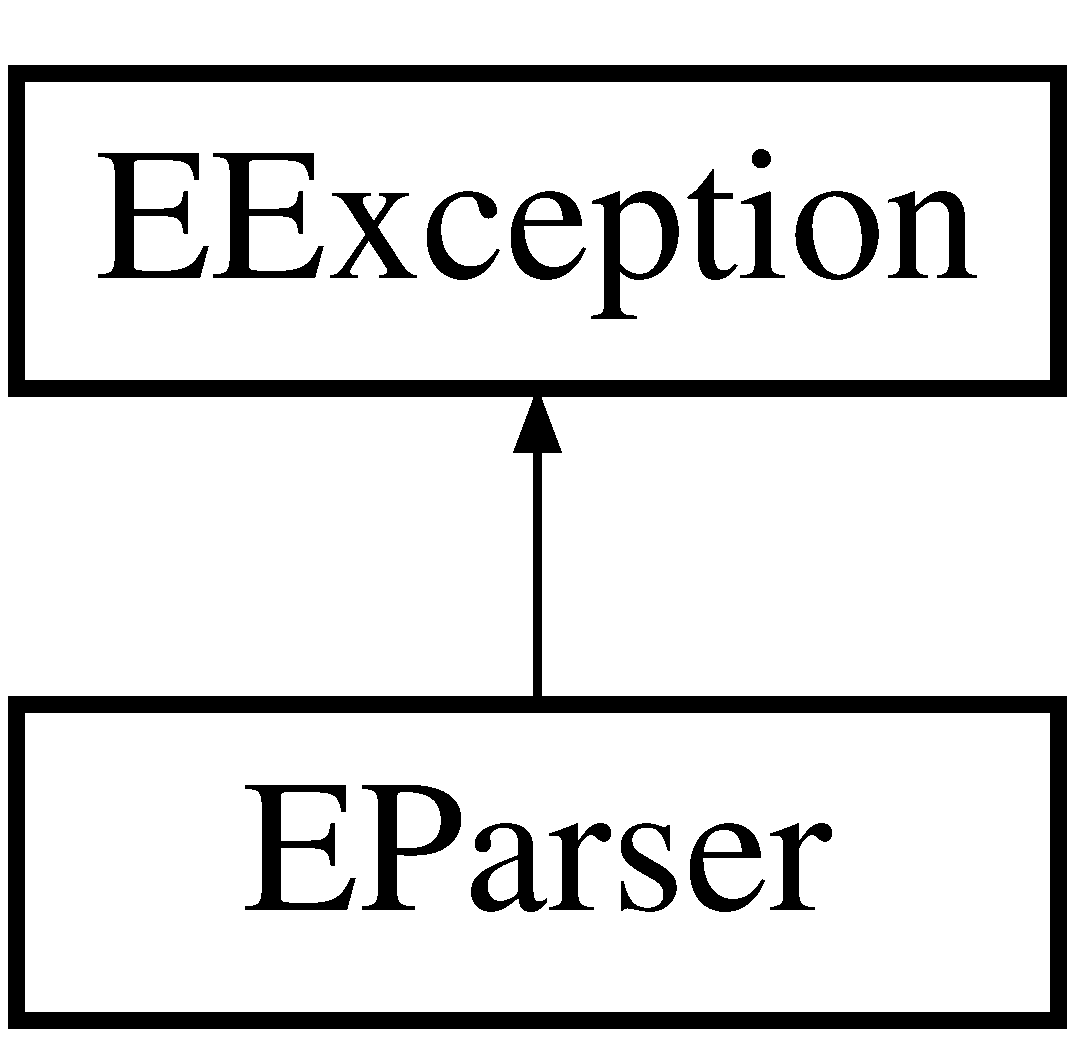
\includegraphics[height=2cm]{classEParser}
\end{center}
\end{figure}
\subsection*{Public Member Functions}
\begin{CompactItemize}
\item 
{\bf EParser} (QString message, int line, const QString s=\char`\"{}\char`\"{})
\item 
{\bf $\sim$EParser} ()
\item 
int {\bf line} ()
\end{CompactItemize}
\subsection*{Protected Attributes}
\begin{CompactItemize}
\item 
int {\bf \_\-line}
\end{CompactItemize}


\subsection{Constructor \& Destructor Documentation}
\index{EParser@{EParser}!EParser@{EParser}}
\index{EParser@{EParser}!EParser@{EParser}}
\subsubsection{\setlength{\rightskip}{0pt plus 5cm}{\bf EParser} (QString {\em message}, int {\em line}, const QString {\em s} = {\tt \char`\"{}\char`\"{}})\hspace{0.3cm}{\tt  [inline]}}\label{classEParser_a0}


\index{EParser@{EParser}!~EParser@{$\sim$EParser}}
\index{~EParser@{$\sim$EParser}!EParser@{EParser}}
\subsubsection{\setlength{\rightskip}{0pt plus 5cm}$\sim${\bf EParser} ()\hspace{0.3cm}{\tt  [inline]}}\label{classEParser_a1}




\subsection{Member Function Documentation}
\index{EParser@{EParser}!line@{line}}
\index{line@{line}!EParser@{EParser}}
\subsubsection{\setlength{\rightskip}{0pt plus 5cm}int line ()\hspace{0.3cm}{\tt  [inline]}}\label{classEParser_a2}




\subsection{Member Data Documentation}
\index{EParser@{EParser}!_line@{\_\-line}}
\index{_line@{\_\-line}!EParser@{EParser}}
\subsubsection{\setlength{\rightskip}{0pt plus 5cm}int {\bf \_\-line}\hspace{0.3cm}{\tt  [protected]}}\label{classEParser_p0}




The documentation for this class was generated from the following file:\begin{CompactItemize}
\item 
{\bf parser.hpp}\end{CompactItemize}
